\documentclass[conference]{IEEEtran}
\IEEEoverridecommandlockouts
\usepackage{cite}
\usepackage{amsmath,amssymb,amsfonts}
\usepackage{algorithmic}
\usepackage{graphicx}
\usepackage{textcomp}
\usepackage{xcolor}
\usepackage{adjustbox}
\def\BibTeX{{\rm B\kern-.05em{\sc i\kern-.025em b}\kern-.08em
    T\kern-.1667em\lower.7ex\hbox{E}\kern-.125emX}}
\begin{document}

\title{Finding Human Emotions from Text Comments\\
{\footnotesize CS4442B Artificial Intelligence 2 Final Project (Undergraduate)}}
\author{\IEEEauthorblockN{Jeongwon Song}
\IEEEauthorblockA{\textit{Department of Electrical and Computer Engineering} \\
\textit{Western University}\\
London, Canada \\
jsong336@uwo.ca}
\and
\IEEEauthorblockN{Jason Koo}
\IEEEauthorblockA{\textit{Department of Electrical and Computer Engineering} \\
\textit{Western University}\\
London, Canada \\
jkoo26@uwo.ca}
}

\maketitle

\begin{abstract}
Texted-based emotion detection has many use-cases as it allows the digitization of human emotion from massive text data generated from social media. This experiment aims to apply transfer learning by leveraging BERT\cite{DBLP:journals/corr/abs-1810-04805}, a transformer-based\cite {DBLP:journals/corr/VaswaniSPUJGKP17} neural architecture which extracts contextual embedding from texts, to detect 27 fine-grained human emotions. The models were trained with one of the largest fined-grained emotion text datasets, GoEmotions \cite{DBLP:journals/corr/abs-2005-00547}. The authors apply two methods to fine-tune pretrained BERT-small\cite{bhargava2021generalization}\cite{DBLP:journals/corr/abs-1908-08962}, a smaller variant of BERT: adding DNN layers that take the pooled output and adding bidirectional GRU layers \cite{DBLP:journals/corr/ChoMBB14} that take sequential embedding. Both models performed very similarly, achieving the same scores up to the third decimal digit. The final models obtained an average ROC score of approximately 0.80 and a macro-F1 score greater than 0.39, thus showing moderate success in detecting appropriate emotions from texts. 
\end{abstract}

\begin{IEEEkeywords}
NLP, Emotion, Emotion-detection, Transfer learning, BERT, GRU, PyTorch, HuggingFace
\end{IEEEkeywords}

\section{Introduction}
With the emergence of deep learning, there have been significant achievements in various sentimental analysis tasks from both research and industrial applications. However, practitioners often simplify the sentiment space, i.e., binary sentiments, preventing sophisticated analyses from text-based data. Fine-grained emotion detection allows for more profound analyses of human sentiments by extracting rigorously categorized emotions from the texts, bringing new opportunities for researchers and engineers in various applications, including chat-based systems, comment analyses, or as a feature to other problems. 

The BERT architecture has gained popularity with its ability to extract contextual embedding using a self-attention mechanism\cite{DBLP:journals/corr/abs-1810-04805}\cite {DBLP:journals/corr/VaswaniSPUJGKP17}. Unlike traditional word embedding techniques, the feature vectors from the BERT are relative to the sentence rather than representing the global word meaning. Many variants of pre-trained BERT models are publicly available, enabling practitioners to build advanced NLP models by simply adding custom layers on top of the pre-trained BERT encoders. In the project scope, we fine-tune BERT-small\cite{bhargava2021generalization}\cite{DBLP:journals/corr/abs-1908-08962}, a smaller variant of BERT, with custom classifier layers which predict human emotions based on the BERT's feature embedding. 

In this experiment, we formulate the emotion detection problem as one versus one, multi-label classification across the 27 different emotions as found in the GoEmotions dataset\cite{DBLP:journals/corr/abs-2005-00547}, one of the largest labelled emotion datasets extracted from Reddit comments. This experiment focuses on two approaches to fine-tuning BERT models: 1) adding DNN classification layers that take the pooled output of BERT and 2) adding bidirectional GRU\cite{DBLP:journals/corr/ChoMBB14} layers that take sequential embeddings of input sequences, then forwards to dense classifier layers. Both models achieved similar results in which the GRU-based network scored a slightly higher micro-F1 compared to the DNN based network. The best model scored an average AUC-ROC over 0.80 and macro-F1 over 0.39, indicating success in detecting emotions from texts. 

\section{Related Work}

Dorottya Demszky et al.\cite{DBLP:journals/corr/abs-2005-00547}, the authors of GoEmotions, compared the performance of fine-tuned BERT and the traditional bidirectional LSTM\cite{https://www.researchgate.net/publication/13853244_Long_Short-term_Memory} with word embedding using the GoEmotions dataset. Dorottya Demszky et al. showed that BERT performed significantly better than LSTM with word embedding by scoring macro-F1 of 0.46 across 27 emotions. . 

Similarly, Alvarez-Gonzalez et al.\cite{https://doi.org/10.48550/arxiv.2109.01900} compared models' performances based on multiple feature extraction methods with the GoEmotions\cite{DBLP:journals/corr/abs-2005-00547} and Vent\cite{DBLP:journals/corr/abs-1901-04856} datasets. Their results showed that the BERT model achieved the best scores among other embedding methods like FastText\cite{DBLP:journals/corr/JoulinGBM16}, TF-IDF and Bag of Words. Alvarez-Gonzalez et al. applied two architectures, first a stacked bidirectional LSTM on top of different embedding layers and second, DNN layers that take the sequential inputs in parallel, pooling the output after the DNN forwards. The BERT models in \cite{https://doi.org/10.48550/arxiv.2109.01900} scored slightly higher F1 than in the original GoEmotion paper\cite{DBLP:journals/corr/abs-2005-00547}. 

\section{Data \& Exploratory Data Analysis}
\subsection{Emotion Taxonomy}
Fine-grained emotion detection is considered a challenging problem due to the ambiguity and complexity of human emotions. The GoEmotions dataset follows a relatively new emotion taxonomy developed by Cowen et al. \cite{DOI:10.1109/IEC47844.2019.8950616} Cowen et al. proposed 27 different emotions found with advanced statistical methods which capture complex semantic space by analyzing human responses from over 2000 video clips. The 27 emotion groups could be further grouped into three more generic emotions, positive, negative, and ambiguous\cite{DBLP:journals/corr/abs-2005-00547}. 

\subsection{Dataset Subsets}
 The Go-Emotions dataset contains 58k selected Reddit comments labeled with 27 different emotions in addition to neutral, where three to five separate raters annotated individual comments providing a total of 221K rows\cite{DBLP:journals/corr/abs-2005-00547}. In this experiment, we removed any ambiguous comments that did not belong to any emotion classes. Any comments with multiple raters were aggregated into a single row. Next, the dataset was reformatted so that comments that did not belong to any emotion class were considered as neutral. After random ordering, the dataset was divided into training, validation and tuning, and test sets. 

\subsection{Imbalance Class}
It is vital to understand the class distribution in the datasets before choosing the metrics to measure the models' performance. Figure 1 shows the proportion of positive labels for each emotion. There are less than 15\% of positive labels for most classes, which must be considered when analyzing the results or setting the classification threshold. Due to a high imbalance in each class, we mainly use F1 score to interpret the models' performance, described in detail the later section.

\begin{figure}[htbp]
\centerline{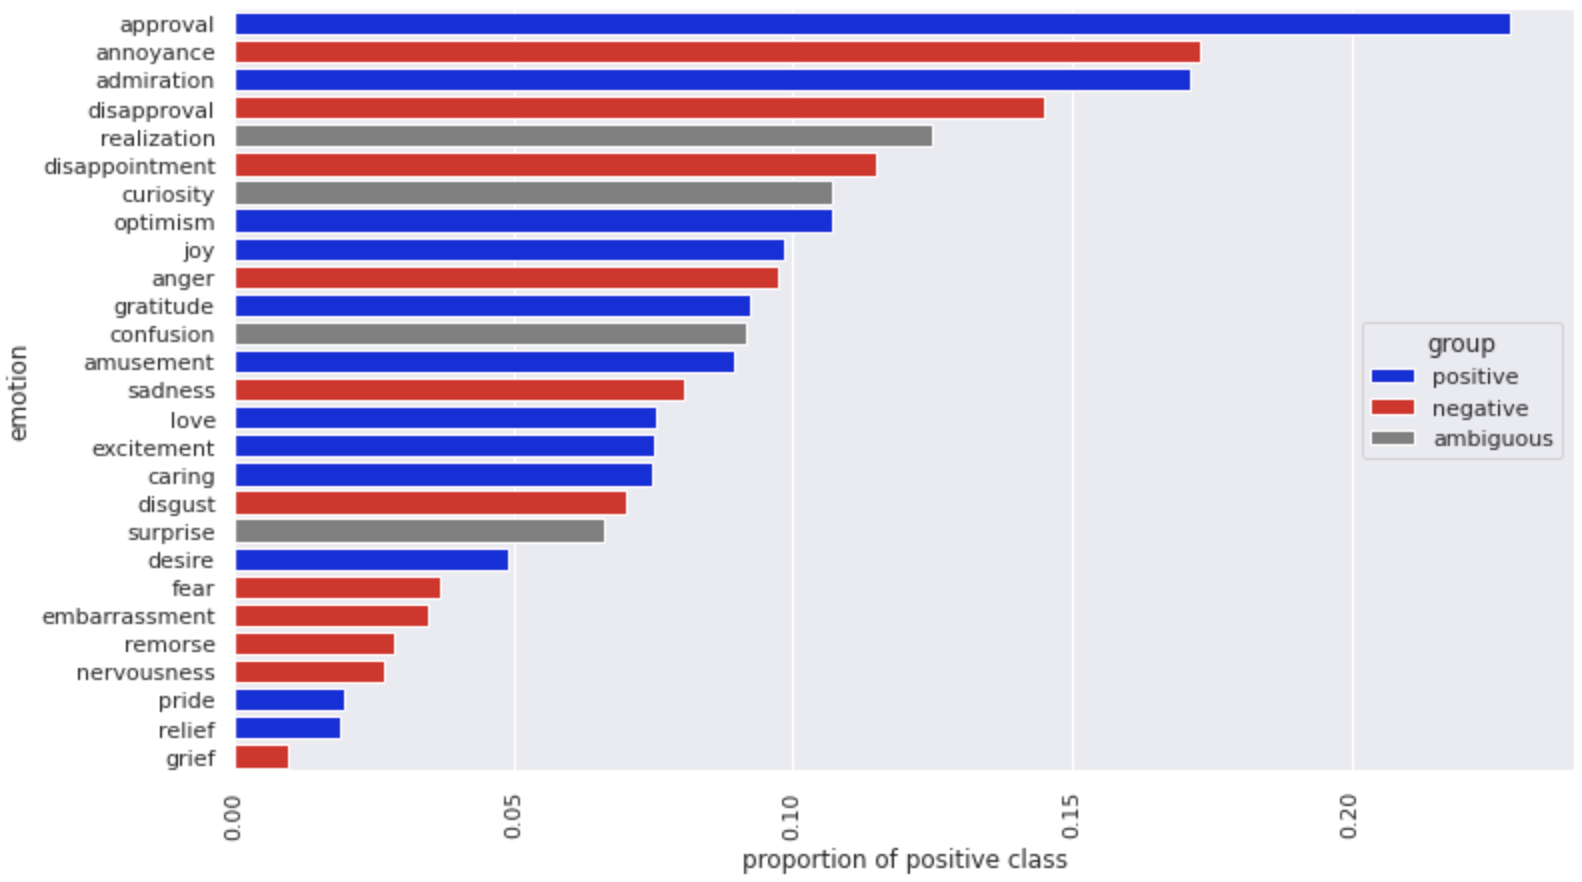
\includegraphics[width=8cm, keepaspectratio]{fig/fine-grained-emotion-proportion-positive.png}}
\caption{Proportion of positive labels for each emotion}
\label{fig}
\end{figure}


\subsection{Relationship between Emotion}
Another interesting factor to consider in the experiment is the correlation between each emotion. Even with advanced emotion taxonomy, a sentence can still covey multiple emotions which could be interpreted differently by both the reader and writer. Through the labelled GoEmotions dataset, we can represent the relationships between different emotions in a more quantifiable way. The high co-occurrence between two emotions in the comments indicates two emotions are more likely to be similar. Hence, we could build a co-occurrence matrix where each column vector of the matrix is normalized except for the diagonal elements resulting in 26-dimensional embedding vectors of each emotion. Figure 4 shows the linear projection of the embedding in the 2D space using Principal Components Analysis. \cite{DBLP:journals/corr/abs-2005-00547} describes similar analyses. 

\begin{figure}[htbp]
\centerline{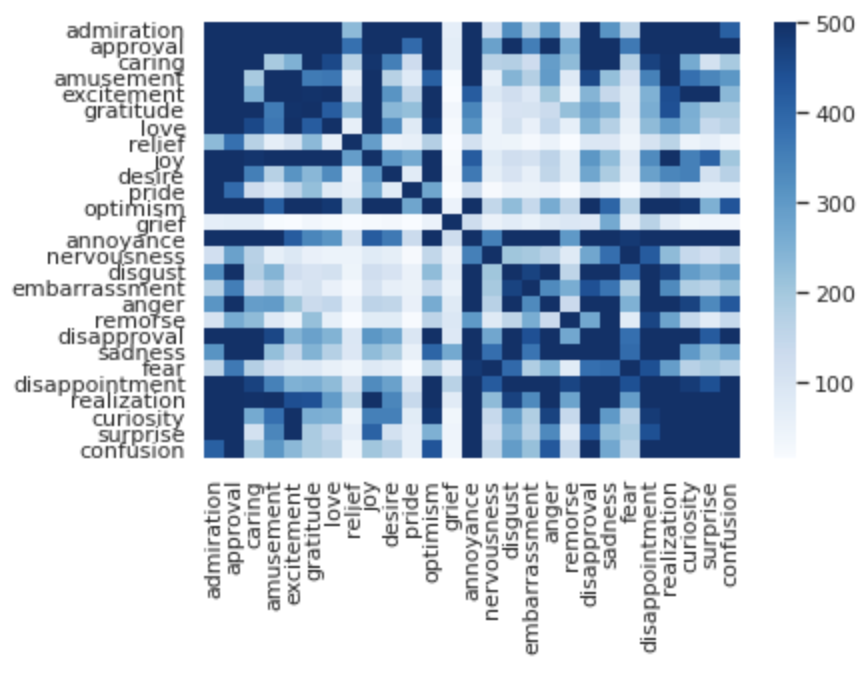
\includegraphics[width=9cm, keepaspectratio,]{fig/cooc-heatmap.png}}
\caption{Co-Occurrence matrix of emotion groups.}
\label{fig}
\end{figure}

\begin{figure}[htbp]
\centerline{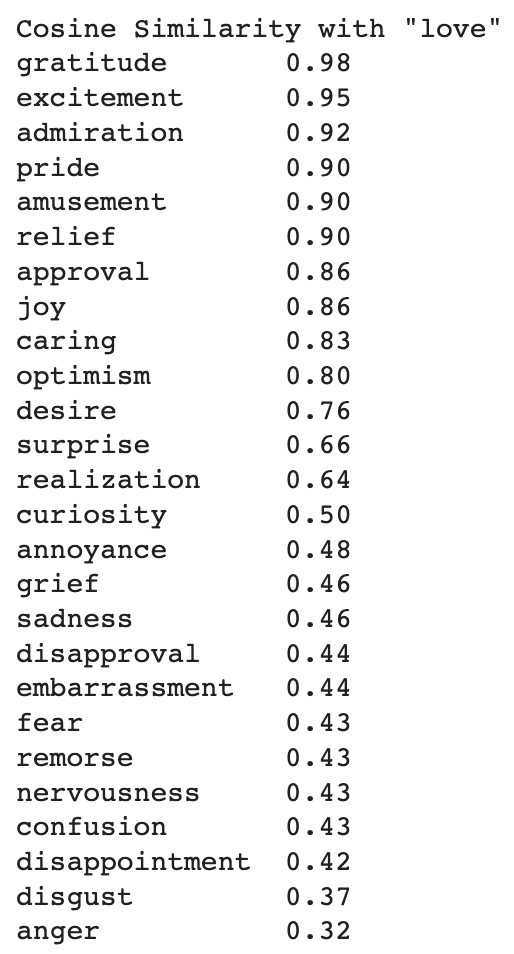
\includegraphics[width=4cm, keepaspectratio,]{fig/love_cosine_sim.png}}
\caption{Cosine similarity between emotions and "love"}
\label{fig}
\end{figure}

\begin{figure}[htbp]
\centerline{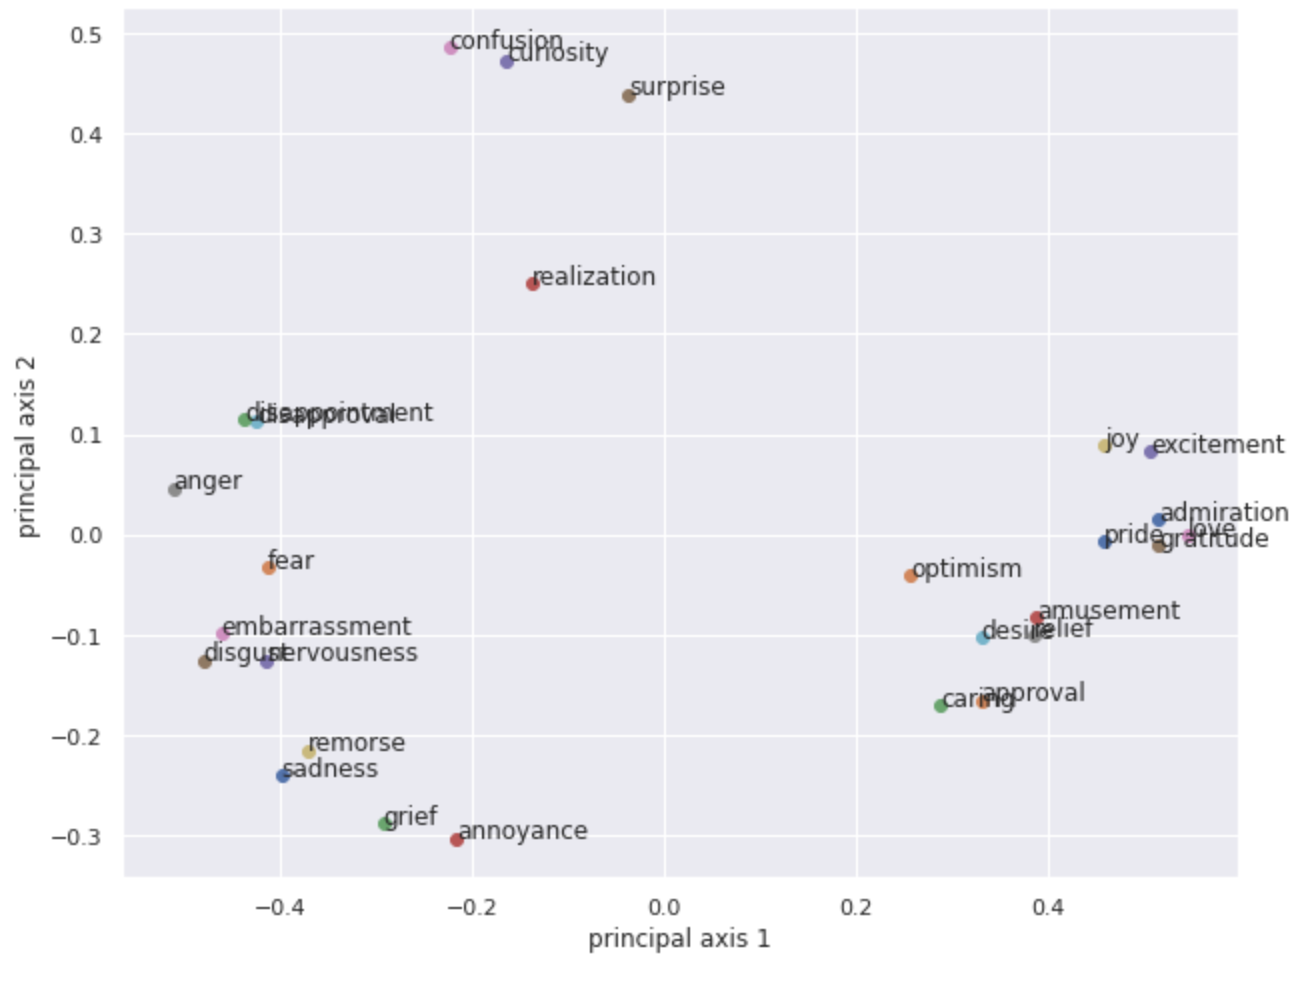
\includegraphics[width=7cm, keepaspectratio,]{fig/covariance-pca.png} }
\caption{Linear Projection of Co-Occurrence matrix of emotion groups.}
\label{fig}
\end{figure}

\section{Data Processing and Feature Engineering}
Data preparation is often the most essential and time-consuming task in many machine learning systems. Especially in text-based features, which require multiple data preparation steps to make text understandable by mathematical models. In this experiment, we utilized the tokenizer published along with the pre-trained BERT-small model\cite{bhargava2021generalization}\cite{DBLP:journals/corr/abs-1908-08962} which provides robust tokenization tasks through common text processing steps. However, to maximize the benefit of transfer learning, it is still essential to ensure that the text data fed to the model does not deviate much from the original text format in which the model was trained. 

\subsection{Text Cleaning}
Since the GoEmotions dataset was extracted from Reddit comments, it contains non-alphanumeric characters, URLs, and spelling mistakes. Below summarizes the text processing steps taken to improve the quality of text before being fed the models. 

\begin{enumerate}
  \item Removing non-alphanumeric or punctuation characters and mapping differently encoded characters. i.e. UTF-8 xE2x80x99(’) and x27('). 
  \item Fixing popular spelling mistakes. The list of popular spelling mistakes is found in Birkbeck spelling error corpus\cite{20.500.12024/0643}. 
  \item Removing URLs, Hashtags, and Emojis with Tweet Preprocessor package\cite{https://github.com/s/preprocessor}.
\end{enumerate}

Furthermore, the pre-built tokenizer performs common text cleaning tasks, including converting to lowercase, splitting punctuation, separating punctuations/contraction, and removing white spaces. 

\subsection{Padding}
BERT\cite{DBLP:journals/corr/abs-1810-04805} requires fixed-length padded sequences and attention masks that indicate whether each token is padding or not. Attention masks allow the model to exempt applying attention to the padding tokens\cite{DBLP:journals/corr/VaswaniSPUJGKP17}. The input sequences are padded with the maximum sequence length. The comments from the GoEmotions dataset have relatively short corpora, where the majority of the texts sequences lengths are below 30. 

\begin{figure}[htbp]
\centerline{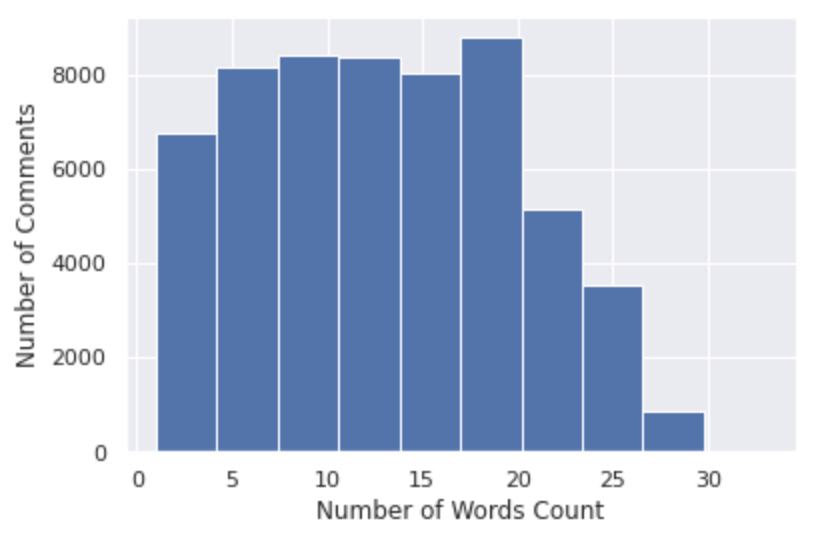
\includegraphics[width=8cm, height=4.5cm]{fig/word-count-per-corpus.png} }
\caption{Distribution of Words Counts}
\label{fig}
\end{figure}

\subsection{Tokenization}
The BERT tokenizer applies the WordPiece algorithm introduced in \cite{DBLP:journals/corr/abs-1810-04805}\cite{DBLP:journals/corr/WuSCLNMKCGMKSJL16} to build the vocabularies by iteratively training the language models with the subwords and combining them with the highest likelihood. This approach allows subword-based tokenization, which mitigates common problems with word-based tokenization, such as large unknown tokens, contractions, and multiple forms of the same words. 

\section{Method}
The project aims to build one versus one multi-label classification models that detect 27 fine-grained emotions using two different neural architectures by fine-tuning BERT-small\cite{bhargava2021generalization}\cite{DBLP:journals/corr/abs-1908-08962}. Each model outputs 27-dimensional vectors where the sigmoid of each element represents the estimated probability of the associated emotion and negative in all categories representing neutral. The results are compared to the performance of similar architectures trained with larger BERT models from \cite{DBLP:journals/corr/abs-2005-00547} and \cite{https://doi.org/10.48550/arxiv.2109.01900}.  

\subsection{Pre-trained BERT and BERT-small}
BERT\cite{DBLP:journals/corr/abs-1810-04805} has gained popularity by providing robust contextual embedding through the self-attention mechanism\cite {DBLP:journals/corr/VaswaniSPUJGKP17}. The original BERT model contains over 12 transformer encoder layers with 768 hidden dimensions and 110M parameters. In this experiment, we use BERT-small with four encoding layers and 512 hidden dimensions \cite{bhargava2021generalization}\cite{DBLP:journals/corr/abs-1908-08962}.

\subsection{Fine Tuning BERT-small With Pooling} 
The original implementation of the BERT model outputs a sequential contextual embedding of the input sequences and the pooled output which is the embedding of the [CLS] token\cite{DBLP:journals/corr/abs-1810-04805}. The [CLS] is a special token added to the beginning of every sequence. The embedding of [CLS] captures the aggregated representation of the whole sequence and is often sufficient in many classification tasks. Thus, we added dense layers with ReLU activation functions on top of the pre-trained BERT model to take the pooled output as features to the classifier units.

\begin{figure}[htbp]
\centerline{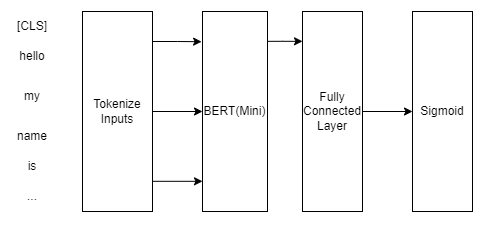
\includegraphics[width=7cm, keepaspectratio,]{fig/bert-pool.png}}
\caption{BERT with Dense}
\label{fig}
\end{figure}

\subsection{Fine Tuning BERT-small With GRU}
Another approach uses sequential embeddings for whole input sequences with bidirectional GRU layers\cite{DBLP:journals/corr/ChoMBB14}. GRU is a variant of RNN published much later than LSTM and is more compactly represented than LSTM\cite{https://www.researchgate.net/publication/13853244_Long_Short-term_Memory}. The performance of LSTM and GRU is often similar, but GRU is considered more efficient and fast trained, whereas LSTM tends to remember hidden states longer than GRU. By stacking two GRU cells where each one takes a sequence from opposite directions, the models learn the hidden state from both directions of the input sequence. The last hidden states of the GRU layers from both directions are forwarded to dense layers, which work as a classifier like previous methods.

\begin{figure}[htbp]
\centerline{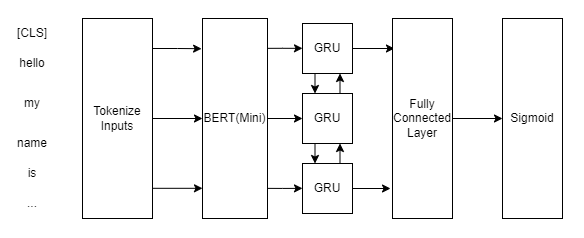
\includegraphics[width=7cm, keepaspectratio,]{fig/bert-gru.png}}
\caption{Tuning BERT with GRU}
\label{fig}
\end{figure}

\subsection{Optimization and Loss Function}

Since each emotion class is considered an individual binary classification task, we use binary cross-entropy as the optimization function. The models are trained with the PyTorch implementation of binary cross-entropy with a log-sum-exponent trick which provides better numerical stability\cite{NEURIPS2019_9015}. 

Adam\cite{https://doi.org/10.48550/arxiv.1412.6980} is an iterative gradient-based optimization algorithm that combines momentum techniques with RMSProps and is considered one of the most popular optimization techniques for deep learning. Adam was often used with L2 regularization to penalize large parameters in the past. However, Ilya Loshchilov et al. showed that applying L2 regularization with Adam is different from weight decaying and is less effective\cite{DBLP:journals/corr/abs-1711-05101}. Hence, Ilya Loshchilov et al. proposed AdamW\cite{DBLP:journals/corr/abs-1711-05101}, a variant of Adam that decouples weight- decaying from optimization steps to apply weight-decaying more effectively on the original Adam algorithm. In this experiment, We used HuggingFace's implementation of AdamW with linear warm-up, which gradually increases the learning rate up to the predefined point and decreases to zero linearly\cite{Wolf_Transformers_State-of-the-Art_Natural_2020}. 

\subsection{Metrics of Interest}
In this experiment, we mainly considered F1 based metrics, including individual F1 score, macro-F1, and micro F1. F1 is the standard metric for measuring the performance of detecting positive classes. F1 scores in multi-classes could be represented in either macro-F1 or micro-F1 in multi-class classification. Macro-F1 is simply averaging the individual F1 scores over 27 emotion classes, whereas micro-F1 calculates F1 by considering the contribution of all classes while computing the metrics.

\section{Experiment Results}
\subsection{Comparing models}
Models were trained with 20 epochs and were saved every half epoch. For each model, the best-performing state was used to compare the performance. Both models performed very similarly up to two decimal places in macro-F1 and micro-F1, shown below.   

\begin{adjustbox}{width=\columnwidth,center}
\begin{tabular}{lrrrr}
    {} & Parameters & M-f1 &  m-f1 & auc-roc \\
    \hline \\
    Baseline(BERT-base)* & 110M & 0.46 & 0.51 & - \\
    CLS Pooled(BERT-small) & 28.8M &  0.395 & 0.453 & 0.798 \\
    GRU-Based(BERT-small) & 28.9M &  0.394 & 0.459 & 0.799
    \hline \\
    \footnotesize{Results as reported by \cite{DBLP:journals/corr/abs-2005-00547}}
\end{tabular}
\end{adjustbox}

Both scored a macro-F1 over 0.39 and a micro-F1 over 0.45, which is reasonable considering similar models trained with the original BERT architecture scored a macro-f1 of near 0.46 with much more parameters in \cite{DBLP:journals/corr/abs-2005-00547} \cite{https://doi.org/10.48550/arxiv.2109.01900}. The GRU-based model scored slightly higher than the DNN based model in micro-F1; however, vice versa in macro-F1.

\begin{figure}[htbp]
\centerline{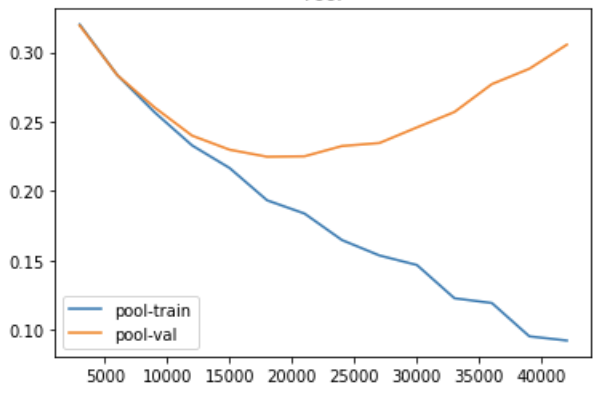
\includegraphics[width=6cm, keepaspectratio,]{fig/val-train-pool.png}}
\caption{Train vs Validation Loss, BERT-small, Pooled}
\label{fig}
\end{figure}

\begin{figure}[htbp]
\centerline{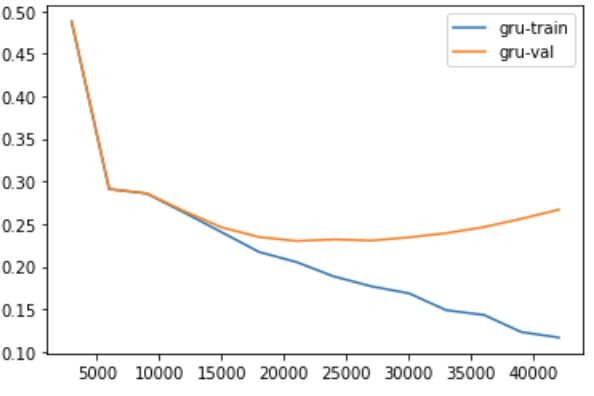
\includegraphics[width=6cm, keepaspectratio,]{fig/val-train-gru.png}}
\caption{Train vs Validation Loss, BERT-small, GRU}
\label{fig}
\end{figure}

\subsection{Positive Prediction Ratio during Training}
It is also interesting to look at recall and the ratio of positive prediction over all predictions i.e. $(TP + FP) /Total$, during training. The ratios of positive labels were low in the dataset, i.e. there are more negatively labelled data than positively labelled. By plotting the ratio of positive predictions and the macro-recall, we see that the models blindly predicted the negative class at the beginning of training until they began to learn and predict with better recall. 


\begin{figure}[htbp]
\centerline{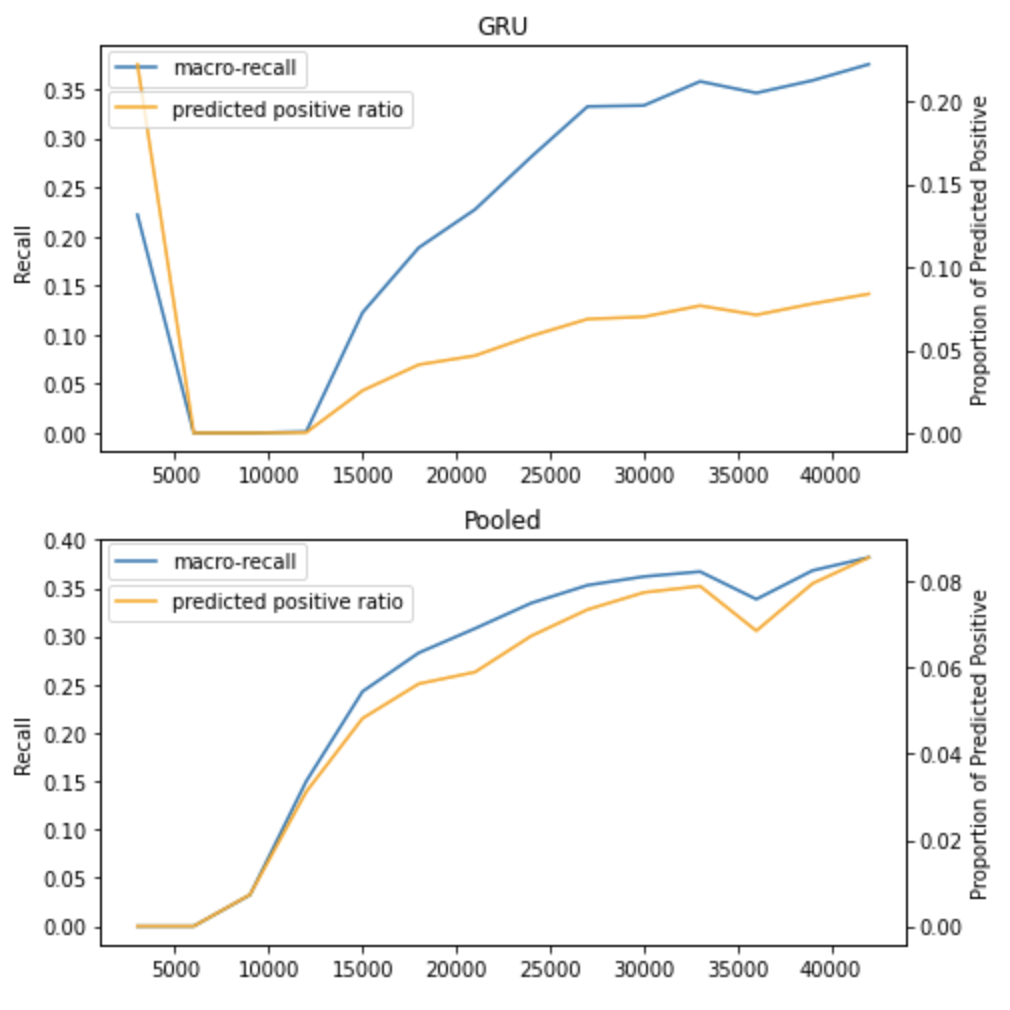
\includegraphics[width=8cm, keepaspectratio,]{fig/recall vs predicted positive ratio.png}}
\caption{Macro Recall vs Predicted Positive Ratio}
\label{fig}
\end{figure}

\subsection{ROC Curve and AUC}
The GRU-based model scored an average AUC-ROC over 0.80, indicating that the models were able to distinguish the positive and negative classes for most emotion classes. Figure 11 shows the ROC curves for all 27 emotion classes. We see that all of the curves are concave over the diagonal line. 

\begin{figure}[htbp]
\centerline{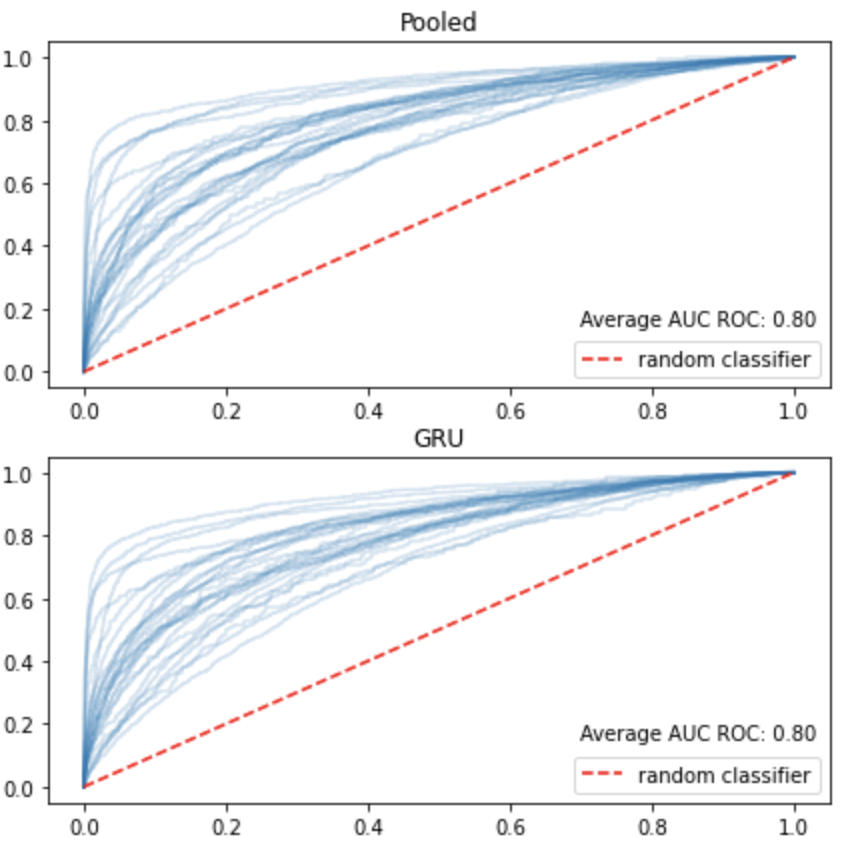
\includegraphics[width=7cm, keepaspectratio,]{fig/roc-curve.png}}
\caption{ Area under the curve ROC }
\label{fig}
\end{figure}

\subsection{Performance Over Emotion Taxonomy}

Looking at the models' performance on individual emotions, we see that F1 scores differ severely across the emotions classes. For example, the models achieved F1 scores over 0.7 in love and gratitude, but they completely failed to detect grief or relief from the text. The Pearson coefficient values between the F1 scores and the percentage of positive labels are 0.46 and 0.43, respectively, for GRU-based and pooled models, indicating models tend to perform better with the more common emotions. However, it is not always the case since few emotions including remorse scored relatively high while rarely occurring in the dataset. 

\begin{center}
\begin{tabular}{lrrr}
\toprule
       Emotion &  Pooled F1 &  GRU F1 &  Positive Ratio \\
\hline
         pride &       0.00 &    0.02 &            0.02 \\
         grief &       0.02 &    0.06 &            0.01 \\
        relief &       0.16 &    0.03 &            0.02 \\
 embarrassment &       0.16 &    0.09 &            0.04 \\
   nervousness &       0.22 &    0.20 &            0.03 \\
   realization &       0.25 &    0.26 &            0.14 \\
        desire &       0.28 &    0.30 &            0.05 \\
disappointment &       0.29 &    0.31 &            0.13 \\
    excitement &       0.32 &    0.34 &            0.08 \\
       disgust &       0.37 &    0.38 &            0.08 \\
        caring &       0.38 &    0.37 &            0.08 \\
     annoyance &       0.40 &    0.44 &            0.19 \\
     confusion &       0.40 &    0.43 &            0.10 \\
      optimism &       0.42 &    0.43 &            0.12 \\
   disapproval &       0.42 &    0.43 &            0.16 \\
      surprise &       0.43 &    0.42 &            0.07 \\
       sadness &       0.43 &    0.43 &            0.09 \\
          fear &       0.46 &    0.45 &            0.04 \\
           joy &       0.46 &    0.44 &            0.10 \\
      approval &       0.46 &    0.44 &            0.25 \\
         anger &       0.47 &    0.46 &            0.10 \\
       remorse &       0.53 &    0.54 &            0.03 \\
    admiration &       0.59 &    0.61 &            0.18 \\
     curiosity &       0.64 &    0.65 &            0.11 \\
     amusement &       0.68 &    0.70 &            0.10 \\
     gratitude &       0.71 &    0.70 &            0.10 \\
          love &       0.74 &    0.73 &            0.08 \\
\bottomrule
\end{tabular}
\end{center}

\section{Conclusion}

We present two approaches to text-based emotion detection with the GoEmotions dataset\cite{DBLP:journals/corr/abs-2005-00547}, one of the largest annotated fine-grained emotion datasets. Our experimentation shows how two different fine-tuned BERT-small\cite{bhargava2021generalization}\cite{DBLP:journals/corr/abs-1908-08962} models behave. The DNN-based model performed slightly better with a macro F1 score of 0.395 than the GRU-based model with a macro F1 score of 0.394. Overall, the models performed very similarly. The DNN-based model tends to converge quicker than the GRU-based model. Although our model performed relatively well, it is still far from the macro F-1 scores achieved by larger models in \cite{DBLP:journals/corr/abs-2005-00547}, and \cite{https://doi.org/10.48550/arxiv.2109.01900}.

As the analyses indicate, GoEmotions datasets contain imbalanced emotion sets, significantly influencing the models' performances in each emotion class. The results are also similar in \cite{DBLP:journals/corr/abs-2005-00547}, and \cite{https://doi.org/10.48550/arxiv.2109.01900}. Moving forward, we could improve the models by collecting more data on the low-performing emotion classes due to insufficient comments and training the models with specific emotions, i.e. grief and pride.

In our experiment, BERT-small was used due to the project scope. However, we could also leverage BERT with more parameters, i.e. BERT-base, to improve the models' performance as shown in the \cite{DBLP:journals/corr/abs-2005-00547}, and \cite{https://doi.org/10.48550/arxiv.2109.01900}. The performances increased drastically from BERT-mini to BERT-small(0.32 - 0.39), and we expect to gain a similar increase with BERT-base\cite{DBLP:journals/corr/abs-1908-08962}.

Furthermore, we could consider distinguishing the emotions annotated by readers and the writers as shown in \cite{https://doi.org/10.48550/arxiv.2109.01900}.
Previous experimentation with the Vent\cite{DBLP:journals/corr/abs-1901-04856} dataset in \cite{https://doi.org/10.48550/arxiv.2109.01900}, showed promising results, surprisingly outperformed humans. The authors of \cite {https://doi.org/10.48550/arxiv.2109.01900} trained the model based on emotions annotated by the writers, in which the model outperformed readers at predicting writer's emotions by 19.9\% relative to macro F1 scores. Additionally, the same model performed better at predicting reader annotated labels despite not having trained specifically for this task. These results indicate a step in the right direction for emotion detection classification. 
\bibliography{main.bib}{}
\bibliographystyle{IEEEtran}


\end{document}
